%==============================================================================
% Sjabloon poster bachproef
%==============================================================================
% Gebaseerd op document class `a0poster' door Gerlinde Kettl en Matthias Weiser
% Aangepast voor gebruik aan HOGENT door Jens Buysse en Bert Van Vreckem

\documentclass[a0,portrait]{hogent-poster}

% Info over de opleiding
\course{Bachelorproef}
\studyprogramme{toegepaste informatica}
\academicyear{2022-2023}
\institution{Hogeschool Gent, Valentin Vaerwyckweg 1, 9000 Gent}

% Info over de bachelorproef
\title{Scholieren met dyslexie van de derde graad middelbaar onderwijs ondersteunen bij het begrijpend lezen van wetenschappelijke artikelen via geautomatiseerde en gepersonaliseerde tekstvereenvoudiging.}
\subtitle{}
\author{Dylan Cluyse}
\email{dylan.cluyse@student.hogent.be}
\supervisor{Lena De Mol}
\cosupervisor{Johan Decorte (Hogeschool Gent); Jana Van Damme (Hogeschool Gent)}

% Indien ingevuld, wordt deze informatie toegevoegd aan het einde van de
% abstract. Zet in commentaar als je dit niet wilt.
\specialisation{AI en data engineering}
\keywords{Gepersonaliseerde tekstvereenvoudiging; dyslexie; natuurlijke taalverwerking}
\projectrepo{https://github.com/dylancluyse/bachelorproef-nlp-tekstvereenvoudiging}

\begin{document}

\maketitle

\begin{abstract}

\end{abstract}

\begin{multicols}{2} % This is how many columns your poster will be broken into, a portrait poster is generally split into 2 columns

\section{Introductie}

Begrijpend lezen behoort tot de belangrijkste vaardigheden in het middelbaar onderwijs. Zo moeten scholieren deze leesvaardigheid onderhouden en bevorderen om het middelbaar onderwijs te kunnen overleven. Dagelijks moeten zij teksten kunnen doornemen en het tekstbegrip ervan onthouden. Scholieren met dyslexie kunnen moeilijkheden hebben bij het begrijpend lezen in het onderwijs. Zo kunnen trage woordbenoeming, hardnekkig letter-voor-letter lezen en moeite bij onregelmatige lettergreepcombinaties obstakels vormen bij deze doelgroep. Daarnaast vraagt het begrijpend lezen van wetenschappelijke artikelen een alsmaar grotere geletterdheid van de lezer. Wetenschappelijk jargon, complexe concepten, veel informatie in een compact formaat, hoog gebruik van meerlettergreperige woorden en cijfermateriaal bij resultaten maken wetenschappelijk artikelen een moeilijke bron om in te zetten in het middelbaar onderwijs. Echter raken scholieren via deze bronnen in contact met wetenschappelijke onderzoek wat het aanleren van kritische vaardigheden met zich meebrengt. Leerkrachten kunnen deze wetenschappelijke artikelen vereenvoudigen op maat van deze scholieren. Dit proces noemt \textit{manual text simplification}. Zij kunnen MTS toepassen door ondersteunende woordenlijsten te maken, zinnen opnieuw te schrijven met een verminderde lexicale en syntactische complexiteit en de tekst te herschrijven als een opsomming of in tabelvorm. MTS past niets aan de oorspronkelijke semantiek aan. Hoewel dit een redmiddel kan zijn voor scholieren bij het begrijpend lezen van een wetenschappelijk artikel, toch is dit een proces dat tijd vergt van de personen die hierop MTS uitvoeren. Dit proces automatiseren met \textit{automatic text simplification} (ATS) is een haalbare taak met een capabel taalmodel, maar huidige toepassingen beschikken over onvoldoende functionaliteiten om gepersonaliseerde ATS aan te bieden. Dit onderzoek moet achterhalen hoe ontwikkelaars gepersonaliseerde ATS-functionaliteiten kunnen aanreiken in de vorm van een prototype.



\section{Experimenten met tools en taalmodellen}

Om deze vraag te beantwoorden, voert het onderzoek drie fasen uit. Allereerst voert het onderzoek een requirementsanalyse uit. Deze requirementsanalyse onderzoekt de functionaliteiten bij huidige tools en toepassingen voor (gepersonaliseerde) ATS. Daarnaast achterhaalt de requirementsanalyse welke MTS-technieken huidige toepassingen ontbreken. De requirementsanalyse wijst de \textit{must-haves} waar het prototype voor gepersonaliseerde ATS over moet beschikken. Vervolgens moet het prototype beschikken over een geschikt taalmodel voor gepersonaliseerde ATS. Na de requirementsanalyse volgt een vergelijkende studie rond beschikbare taalmodellen om gepersonaliseerde ATS te kunnen realiseren. Het doel van deze onderzoeksmethode is om de beschikbare taalmodellen op HuggingFace en het GPT-3 taalmodel tegenover elkaar te plaatsen. Twee wetenschappelijke artikelen en twee MTS-vereenvoudigde teksten dienen als testmateriaal. Hier wordt gekeken welk taalmodel rekening houdt met gepersonaliseerde ATS, met gelijke kwaliteiten als MTS.

\section{Ontwikkeling van een prototype}

Het prototype maakt gebruik van vrij beschikbare technologieën en programmeertalen, zoals HTML/CSS, Python en Het prototype bestaat uit twee componenten. Enerzijds kan het prototype een ondersteunend middel bieden aan scholieren met dyslexie, door een wetenschappelijk artikel in een aanpasbaar formaat aan te bieden. Daarnaast kunnen scholieren aanpassingen aan de tekst maken, zoals weergegeven in figuur \ref{img:figure-1}. Anderzijds kunnen leerkrachten een vereenvoudigde versie van een wetenschappelijk artikel laten maken met het prototype. Hier kan de leerkracht parameters meegeven, waaronder de opmaakopties en de vereenvoudigingen die de tekst moet aannemen, zoals weergegeven in figuur \ref{img:figure-2}.

\begin{center}
	\captionsetup{type=figure}
	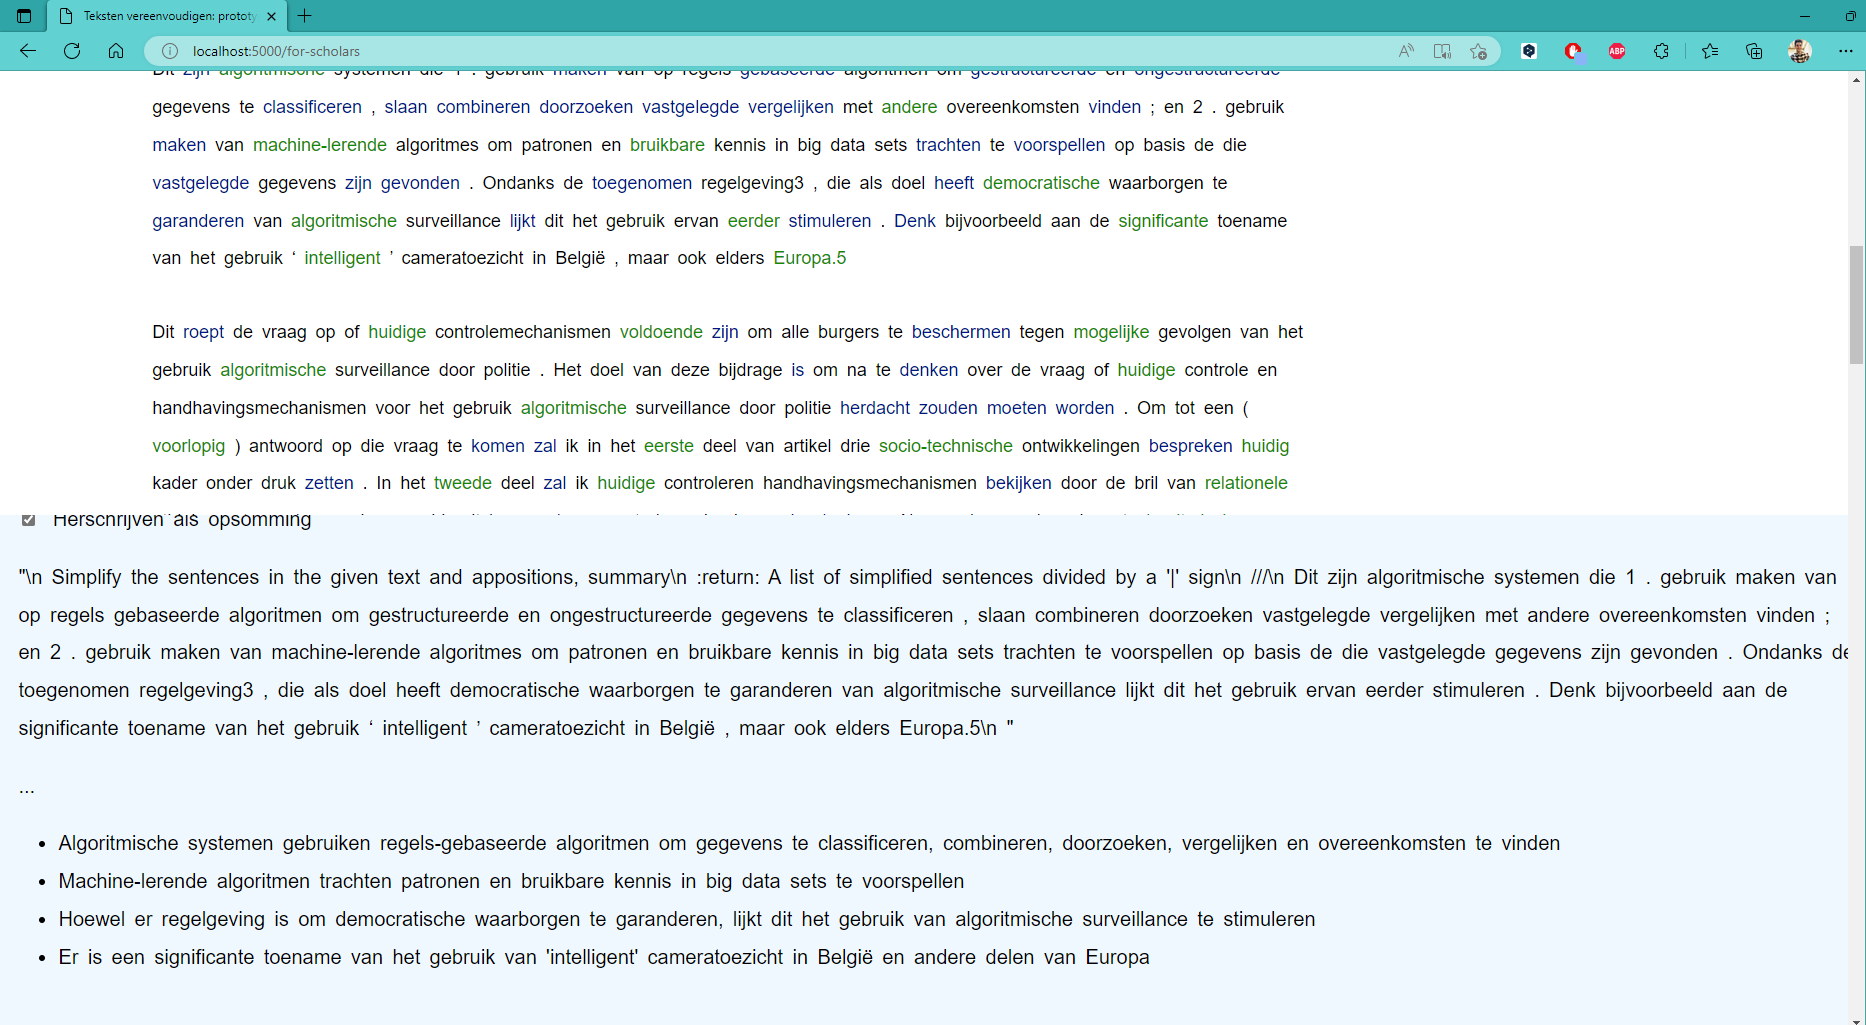
\includegraphics[width=1.0\linewidth]{figures/proto-opsomming-2.png}
	\captionof{figure}{Voorbeeldweergave van het scholierencomponent. De scholier selecteert een tekst en vraagt voor een opsomming (met eenvoudige woordenschat) van de gemarkeerde tekst.}
	\label{img:figure-1}
\end{center}


\begin{center}
	\captionsetup{type=figure}
	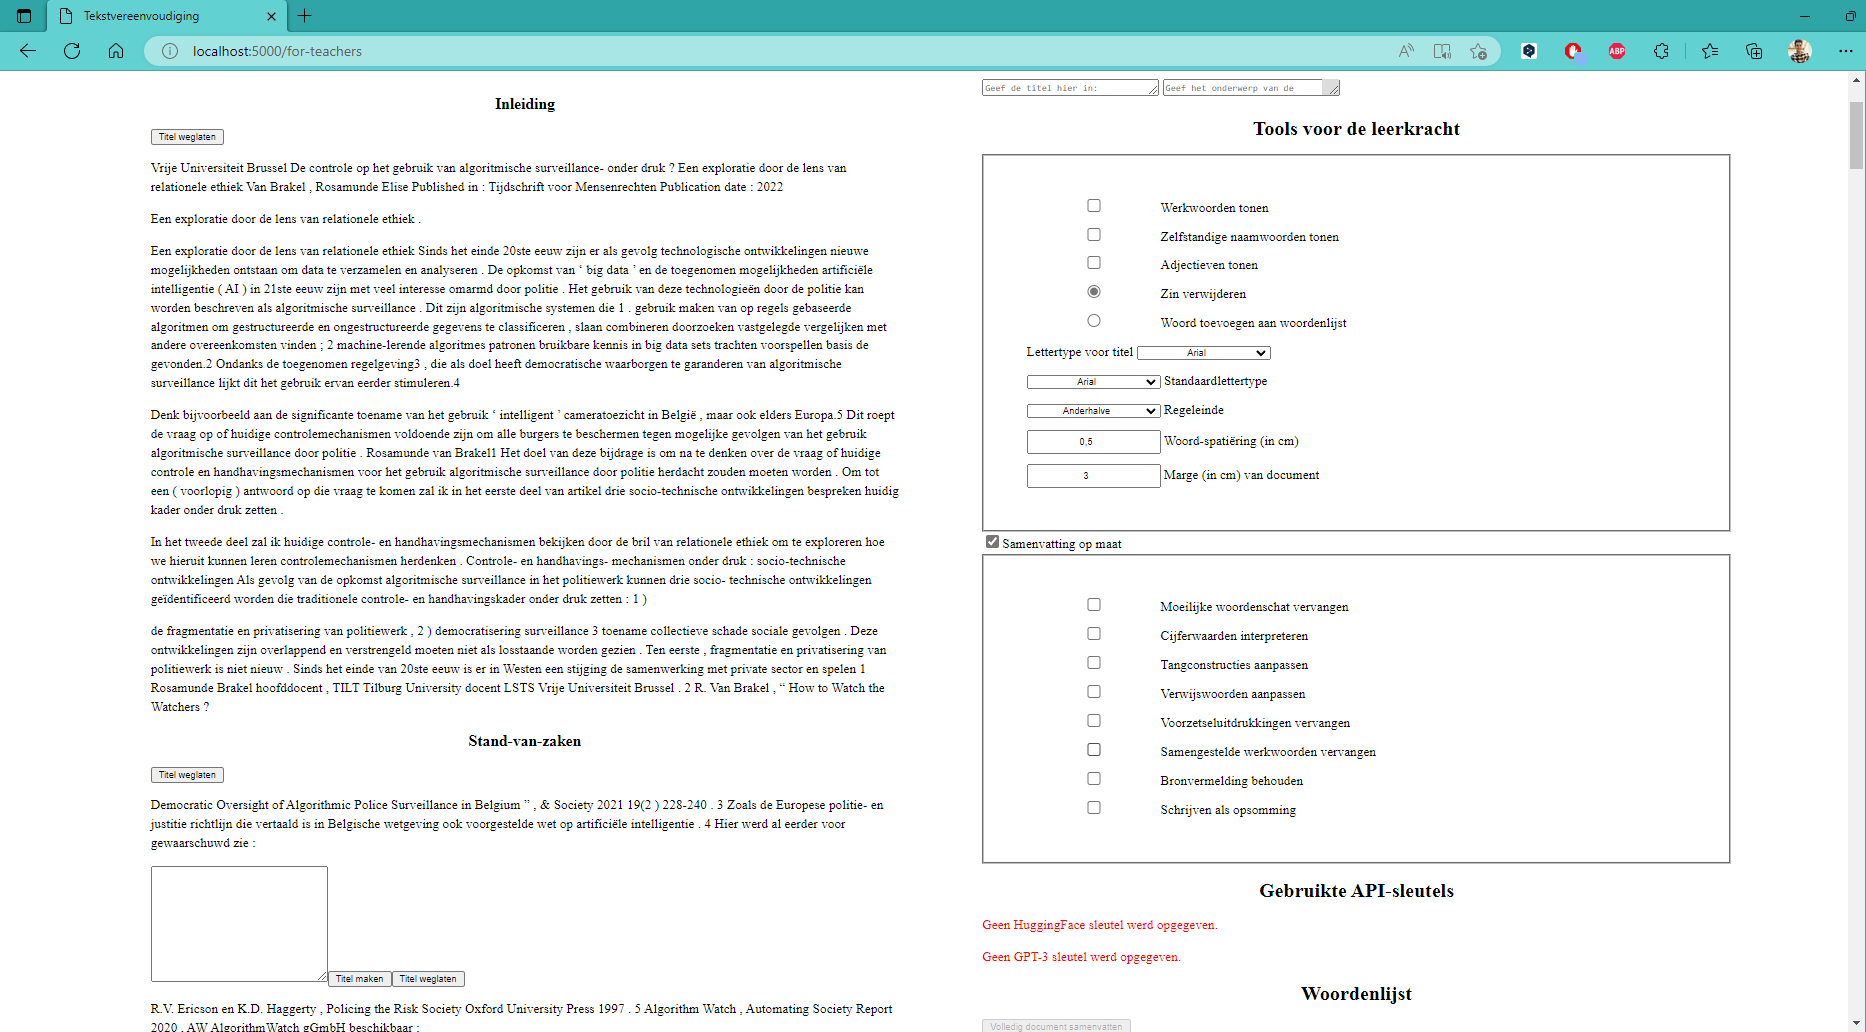
\includegraphics[width=1.0\linewidth]{figures/proto-lerarencomponent.png}
	\captionof{figure}{Voorbeeldweergave van het lerarencomponent. De leerkracht kan een wetenschappelijk artikelDe scholier selecteert een tekst en vraagt voor een opsomming (met eenvoudige woordenschat) van de gemarkeerde tekst.}
	\label{img:figure-2}
\end{center}

\section{Conclusies}

Het prototype voldoet aan alle \textit{must-have} functionaliteiten om gepersonaliseerde ATS aan scholieren met dyslexie te kunnen bieden voor het begrijpend lezen van wetenschappelijke artikelen.

\section{Toekomstig onderzoek}
Verder onderzoek naar de toepassing van AI via een API, zoals het GPT-4 taalmodel, is noodzakelijk en kan baanbrekend zijn voor de onderwijssector. Dit onderzoek kan zich richten op doelgroepinschattingen via prompts en het potentieel van de combinatie van GPT-3 en textit{full-text-search}-technologieën. Daarnaast is er behoefte aan onderzoek naar de verschillen tussen taalmodellen getraind op wetenschappelijke artikelen en taalmodellen getraind op algemene data. Tot slot kunnen logopedisten en studenten in deze richting het prototype gebruiken om verder onderzoek uit te voeren naar de effecten van gepersonaliseerde ATS bij scholieren met dyslexie in de derde graad van het middelbaar onderwijs. 

\end{multicols}
\end{document}